\hypertarget{validating-the-cpu-in-prototyping-hardware}{%
\chapter{Validating the CPU in Prototyping
Hardware}\label{validating-the-cpu-in-prototyping-hardware}}

In this step, we will test the CPU and application, which were generated
in the previous steps, on a FPGA prototyping system. For this purpose,
we will use the XUPV5-LX110T Prototyping Board from Xilinx shown in Figure \ref{fig:fig61}.
\begin{figure}[!htb]
	\centering
	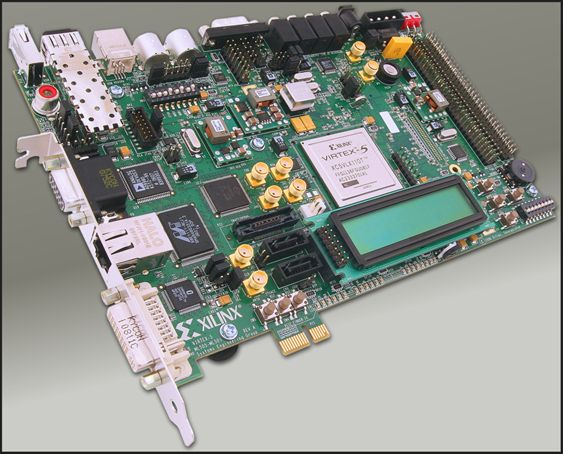
\includegraphics[width=0.9\textwidth]{src/images/6-1.png}
	\caption{XUPV5-LX110T Prototyping Board from Xilinx \cite{HWAFX}}
	\label{fig:fig61}
\end{figure}
\hypertarget{creating-the-ise-project}{%
\section{Creating the ISE Project}\label{creating-the-ise-project}}

ISE (also called Project Navigator) is a program from Xilinx to support
the whole tool-flow from managing your source files during synthesis,
map, and place \& route until finally uploading the design to the FPGA
board.

Start ISE by just executing ``\emph{ise \&''} in your ASIP project
directory

If you do not already have a project for your current CPU, then create a
new one: Select \emph{File} Menu \textgreater{} \emph{New~Project}. As
``\emph{Project Path''} you should choose your ASIP Meister Project
Directory (e.g. ``\emph{ASIPMeisterProjects/browstd32/'')} and as
``\emph{Project Name''} you can choose something like
``\emph{ISE\_Framework}''. This ``\emph{Project Name''} will then
automatically be added as new subdirectory to your chosen \emph{Project
Directory}. In the upcoming window ``\emph{Device Properties}'', you
have to adjust the values to the data shown in Figure \ref{fig:fig62}. Afterwards just press \emph{Next
\textgreater{} Next \textgreater{} Finish} to create an empty project
for your CPU. The device settings are needed to make sure, that the map,
place and route tools know exactly the type of the target FPGA. For
example, you will have a project with following project settings:
\begin{lstlisting}
Project Name: ISE_Framework
Project Path: home/asip04/ASIPMeisterProjects/browstd32/ISE_Framework
Device Family: Virtex5
Device: xc5vlx110t
Package: ff1136
\end{lstlisting}
\begin{figure}[!htb]
	\centering
	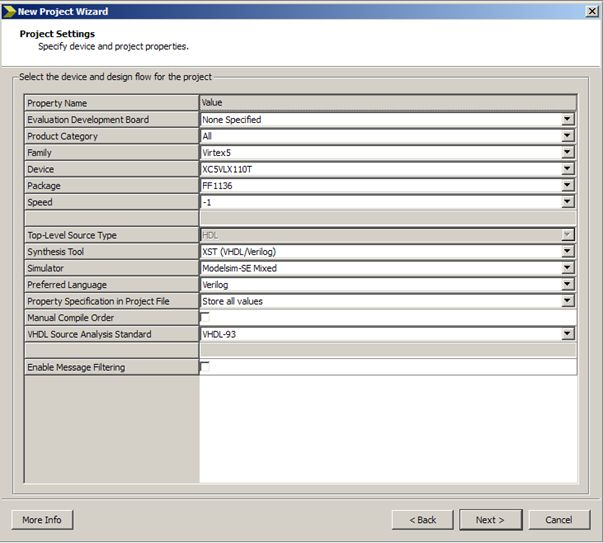
\includegraphics[width=0.9\textwidth]{src/images/6-2.png}
	\caption{ISE Device Properties}
	\label{fig:fig62}
\end{figure}
\hypertarget{adding-source-files-to-ise-project}{%
\section{Adding Source Files to ISE
Project}\label{adding-source-files-to-ise-project}}

Now you have to add the needed VHDL and constraint files to your ISE
project, by right clicking on the XC5VLX110T-1ff1136 entry of your
Sources View (at the upper left inside your ISE Window, see Figure \ref{fig:fig63} \&
Figure \ref{fig:fig64}) and choosing ``\emph{Add Copy of
Source}''. After ISE has analyzed the type of the files, press OK.
Adding a copy of the source has the advantage, that you can locally
modify the files and that the CPU files in your ISE project are not
overwritten, when you modify your ASIP Meister Project for testing
purpose.

There are three types of files that are needed for a hardware
implementation:

\begin{itemize}
\item
  CPU VHDL Files
\item
  Framework Files
\item
  Framework IP cores
\end{itemize}
\begin{figure}[!htb]
	\centering
	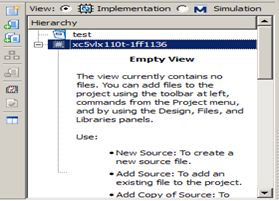
\includegraphics[width=0.7\textwidth]{src/images/6-3.png}
	\caption{Add Sources}
	\label{fig:fig63}
\end{figure}
\begin{figure}[!htb]
	\centering
	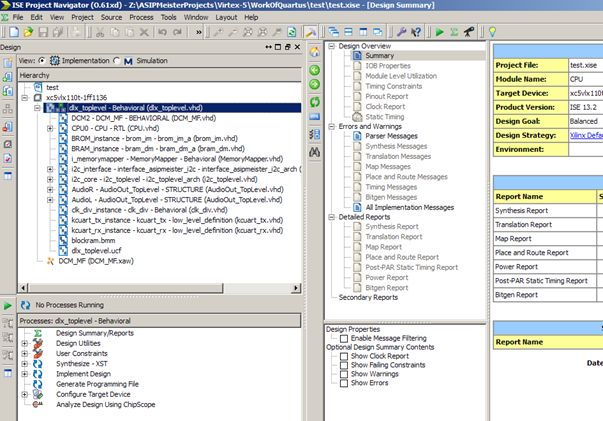
\includegraphics[width=0.9\textwidth]{src/images/6-4.png}
	\caption{ISE Project Overview}
	\label{fig:fig64}
\end{figure}
\textbf{CPU VHDL Files} have been generated using ASIP Meister and they
can be found in the \emph{meister/\{CPU-Name\}.syn} directory, as
explained in Chapter~2.2.2.

\textbf{Framework Files} are important for the connection between CPU,
Memory, UART, and all other components. They are predesigned for this
laboratory and they are available in
\emph{/homeces-asip00/­ASIPMeisterProjects/­TEMPLATE\_PROJECT/­ISE\_Framework}.
The framework consists of the following three types of file and all of
them have to be added to the ISE project.

\begin{itemize}
\item
  \begin{quote}
  The VHDL files describe how all components are connected together.
  \end{quote}
\item
  \begin{quote}
  The UCF file describes the user constraints (e.g., which I/O pins
  should be used for a signal, which clock frequency is requested etc.).
  \end{quote}
\item
  \begin{quote}
  The BMM file contains a description of the memory buildup for
  instruction- and data-memory for the CPU. Out of this file
  \emph{\ldots\_bd.bmm} file will be generated while implementation and
  this file is then used to initialize the created bitstream with the
  application data, as explained in Chapter~6.4.
  \end{quote}
\end{itemize}

\textbf{IP cores} are used within the framework, e.g. memory blocks for
instruction- and data-memory or FIFOs for the connection to the LCD.
These IP cores are not available as VHDL source code, but instead they
are available as pre-synthesized net lists. These files just have to be
copied into the directory of your ISE project (no need to actually add
them to the project) and then they will be used during the
implementation step. The needed files (*.edn, *.ngc) are available in
\emph{/home/ces-asip00/­ASIPMeisterProjects/­TEMPLATE\_PROJECT/­ISE\_Framework/­IP\_­Cores}.
Note: The files {inside} the IP\_Cores directory have to be copied to
your ISE Project Directory. It is not sufficient to copy the full
IP\_Cores directory!

After you have added/copied all needed files to your ISE
project/directory, your main window should look similar to the
screenshot shown in Figure \ref{fig:fig64}. In the
sources sub window you can see all the source files and how they are
structured, i.e. according to the file instantiated by other file.

\hypertarget{synthesizing-and-implementing-the-ise-project}{%
\section{Synthesizing and Implementing the ISE
Project}\label{synthesizing-and-implementing-the-ise-project}}

In the Processes sub window in the lower left corner of
Figure \ref{fig:fig64}, the possible actions for each
kind of file is shown. To synthesize and to implement your project you
have to choose your VHDL-Toplevel in the Sources sub window
(``\emph{dlx\_Toplevel}'' in the figure) and afterwards you have to
double click ``\emph{Generate Programming File}'' in the Processes sub
window. This will finally create the .bit file that can then be
initialized with your CPU instruction- and data-memory and afterwards be
uploaded to the FPGA prototyping board.

The whole process of synthesizing and implementing the design is
subdivided into several steps that can be seen, if you click on the plus
sign in the processes sub window. After the completion of each step, an
update of the \emph{FPGA Design Summary} will be shown in the
corresponding sub window in the upper right corner. For example, the
device utilization (i.e. the size of your CPU plus the framework) will
be shown for the different types of elementary hardware available on the
FPGA (e.g. clocks, logic, BRAMs). This is a first hint, how big your CPU
actually is, but as it will be explained in Chapter~6.5, these values
are not completely accurate, as they not only include the CPU, but also
include the Framework, which consists of many different components.

While synthesizing and implementing the design, many warnings will be
printed. These warnings (unless created by a user modification, e.g. in
the CPU) can be ignored. However, it should be mentioned, that it is
very helpful to understand the meaning of these warnings when you are
looking for a reason why something is working unexpected in hardware.
The challenge here is, that the CPU and the IP cores create plenty of
warnings, thus it is hard to locate the serious warnings.

\hypertarget{initializing-fpga-internal-memory-with-your-application}{%
\section{Initializing FPGA Internal Memory with your
Application}\label{initializing-fpga-internal-memory-with-your-application}}

After you have finished the synthesizing and implementation step, you
receive a bitstream of your ISE project that includes your CPU connected
to an internal memory inside the FPGA. Now you have to initialize this
FPGA internal memory (called Block RAM or BRAM) with your application
instruction- and data memory to execute your program on your CPU. This
initialization can be done inside the bitstream itself, i.e. before
uploading the bitstream to the FPGA board.

To initialize the bitstream with your application, you need your
application as \emph{TestData.IM} and \emph{TestData.DM} files, created
with ``\emph{make sim}'' or ``\emph{make dlxsim}'' as explained in
Chapter~2.3. However, compared to simulation with dlxsim or ModelSim you
have to consider, that you have a limited amount of memory on the FPGA
and therefore you have to adjust the position were the stack starts. For
the usual simulation, the stack can start at some address e.g, 0xFFFFC
and is growing downwards. For hardware execution, this address is too
big. For the current hardware prototype, you should use 0xEFFC. You can
adjust the place where the stack will start in the file
\emph{/home/ces-asip00/epp/mkimg/Makefile} by adjusting
\emph{STACK\_START\_FPGA} variable. This \emph{Makefile} is accessed
from your local application \emph{Makefile} located in the directory of
your application (like
\emph{/home/ces-asip00/­ASIPMeisterProjects/­TEMPLATE\_PROJECT/­Applications/­TestPrint/Makefile})
and it is evaluated every time you execute this local \emph{Makefile}.
Here you can configure the address of the stack start. To work in
hardware this value depends of the size of the available memory in
hardware. For our current prototype, ``0xEFFC'' is the correct value. In
case of FPGA, this parameters is set to STACK\_START\_FPGA.

After the \emph{TestData}-files for your application are created (see
above and Chapter~2.3) and the bitstream of your ISE project is created
(see Chapter~6.1 and Chapter~6.3) you can initialize the bitstream with
your application data by executing ``\emph{make fpga}'' in your
application subdirectory. This script will create two new files in
\emph{BUILD\_SIM} subdirectory of your application like
\emph{DirectoryName.mem} and \emph{DirectoryName.bit}. The .mem file
contains a memory dump for data and instruction memory and is only a
temporary file. The bit file is the final bitstream of your specific CPU
surrounded by the framework, and with your application initialized to
the BRAM. You have to configure the ISE project that you want to use in
the ``\emph{env\_settings}'' as ``\emph{ISE\_NAME}''. The bitstream in
this directory will be used to create the application-initialized
bitstream.

\hypertarget{uploading-the-bitstream-to-fpga-board}{%
\subsection{Uploading the Bitstream to FPGA
Board}\label{uploading-the-bitstream-to-fpga-board}}

After you have created the final bitstream with the initialized BRAM,
you can upload this bitstream to the FPGA Board. At first, you have to
turn the FPGA Board on.
\begin{figure}[!htb]
	\centering
	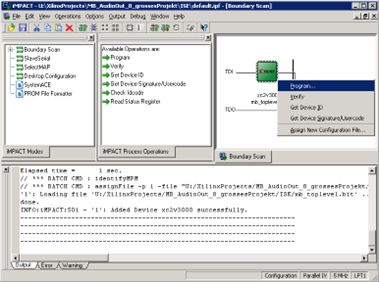
\includegraphics[width=0.9\textwidth]{src/images/6-5.png}
	\caption{Uploading the Bitstream with iMPACT}
	\label{fig:fig65}
\end{figure}
After the FPGA Board is running, you have to connect the FPGA to the PC
and then initialize it with your Bitstream. Therefore, the software
iMPACT from Xilinx, shown in Figure 6-5 is used. If you try to start
iMPACT you will receive an error message, complaining about the
project-/ and the working directory (because you are not an
administrator on this PC). Therefore, right-click the symbol and choose
``\emph{properties}''. Then configure the working directory to
``\emph{U:}'' (this is your mounted Linux-server home). Afterwards you
can start iMPACT. Create a new project (no need to `save' and `load' a
project) and choose the default point ``\emph{Configure Device using
Boundary Scan (JTAG)}''. You should see a JTAG chain with one device
(the FPGA) as shown in Figure 6-5. Assign the bitstream of your
application subdirectory
(ASIPMeisterProjects/browstd32/Applications/...) to the Xilinx FPGA
device. To reactivate this menu point in a later run without restarting
iMPACT, just right-click on the Xilinx device and choose ``\emph{Assign
New Configuration File}''. To program the Xilinx device (i.e. the FPGA)
choose ``\emph{Program}'' as shown in Figure 6-5 and confirm the dialog
without any changes with ``OK''.

Instead of using graphical iMPACT tool for uploading the bitstream to
the FPGA, you can use your Makefile ``\emph{make upload}'' in your
application subdirectory to upload the combined bitstream to the FPGA.
This will automatically scan and program the FPGA.

\hypertarget{initializing-and-using-the-external-sram}{%
\subsection{Initializing and Using the External
SRAM}\label{initializing-and-using-the-external-sram}}

The size of the BlockRAM (i.e. FPGA-internal RAM; at most 192 Kbyte for
our FPGA, but something is used in the Framework for FIFOs etc.) is
limited. This is especially problematic if a huge amount of input-data
is to be used for an application. Therefore, we have provided external
SRAM to the Board, altogether four MB SRAM for IM and four MB SRAM for
DM respectively. Our provided ISE Framework (see Chapter~6.1) provides
the connection between the CPU and the SRAM. However, before the SRAM
can be used it has to be initialized. Currently the SRAM initialization
is unexpected slow. Therefore, whatever you want to test on the FPGA
board, test a BlockRAM version first. The provided ISE Framework still
provides the connection to the BlockRAM additionally. You just have to
follow the above tutorials (Chapter~6.4 and 6.4.1) but do not forget to
configure \emph{STACK\_START\_FPGA} in the Makefile to 0xEFFC. To use
the SRAM, follow the following tutorial:

\begin{itemize}
\item
  You have to compile the \emph{bootloader.c} application (you can find
  it in
  \emph{/home/ces-asip00/­ASIPMeisterProjects/­TEMPLATE\_PROJECT/­Applications/­Bootloader/})
  with ``\emph{make sim}'' and initialize the bitstream with the
  application using ``\emph{make fpga}''. The resulting bit file
  contains the bootloader application in the FPGA internal BlockRAM.
\item
  You have to compile the user application (i.e. the one that you
  actually want to run from the SRAM) with the \emph{STACK\_START\_FPGA}
  configured to 0xFFFFC (in the Makefile; instead of 0xEFFC for BRAM).
  Note that, besides the normal \emph{TestData.IM} and
  \emph{TestData.DM} additionally the files \emph{TestData.IM\_uart.txt}
  and \emph{TestData.DM\_uart.txt} are also created in the
  \emph{BUILD\_SIM} subdirectory.
\item
  You have to start the ``\emph{dlx\_uart.ht}'' file under windows,
  which will open the MS Windows HyperTerminal with the correct settings
  (\emph{Bits per Second=230400, Data Bits=8, Parity=None, Stop Bit=1,
  Flow Control=None}). You can find ``\emph{dlx\_uart.ht}'' in
  \emph{/home/ces-asip00/­ASIPMeisterProjects/­TEMPLATE\_PROJECT/­Applications/­Bootloader}).
  However, you may have to adapt the configured COM port, depending on
  which port you are connected to the FPGA (see
 Figure \ref{fig:fig66}). Under, Ubuntu, you can start
  HyperTerminal by typing ``\emph{hterm \&}'' and can configure the
  settings as mentioned before. After that, you have to click the
  ``\emph{connect}'' button to open the connection. Opening the
  connection always works without error message, but you have to make
  sure that the FPGA board is connected to the PC where you are running
  the HyperTerminal via UART.
\item
  Now configure the FPGA Board to run with 40 MHz (see point (9) in
  Figure \ref{fig:fig66}) and upload the bootloader
  bit-file (created in first step) with iMPACT. The UART port on the
  FPGA is configured to work with 40 MHz and if you use a faster or
  slower frequency, then you will not see the correct output via UART.
  The bootloader will prompt on the UART-Console for initializing the
  SRAM. It will ask for three things (you have to answer with pressing
  `y' or `n'): Initialize IM, Initialize DM, and Start Application.
\item
  To initialize IM or DM you have to select `y' and then use the
  HyperTerminal menu ``\emph{Übertragung}'' ``\emph{Textdatei senden}''
  to upload the file \emph{TestData.IM\_uart} or
  \emph{TestData.DM\_uart}.
\item
  If you do not start the application in the IM-SRAM (pressing `n' when
  asked) OR when the IM-SRAM application is finished OR when you press
  the reset button THEN you will come back to the bootloader.
\end{itemize}
\begin{figure}[!htb]
	\centering
	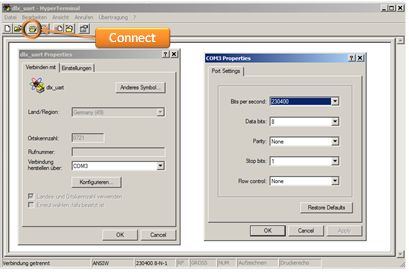
\includegraphics[width=0.7\textwidth]{src/images/6-6.png}
	\caption{Hyper-terminal settings}
	\label{fig:fig66}
\end{figure}
\hypertarget{hardware-specific-limitations-of-the-application}{%
\subsection{Hardware Specific Limitations of the
Application}\label{hardware-specific-limitations-of-the-application}}

Many kinds of applications can be simulated with dlxsim or ModelSim, but
to be able to be executed in hardware, there are some further
limitations, which have to be considered. The most obvious point is the
limitation of the available memory for instructions and data on the
hardware prototype. Currently there are 16 KB for instruction and 16 KB
for data memory available. A part of the ``\emph{make fpga}'' script
will test, whether the your application binary including program and
static data memory fits into these memory portions, but for dynamic
requested data memory, like the stack which is growing with the number
of nested function calls cannot be tested at compile time. If you need
more memory, you have to use the SRAM instead (see Chapter~6.4.2).

Another point is that there are more NOP instructions needed for
hardware execution than for simulation. Therefore, ``Makefile'' file has
to be adjusted accordingly as explained in Chapter~6.4.

The current connection to the data memory does only support word access
to the data memory. Thus, the only supported memory access assembly
instructions are ``\emph{lw}'' and ``\emph{sw}''. The assembly
instructions ``\emph{lb}'', ``\emph{lbu}'', ``\emph{lh}'',
``\emph{lhu}'' actually work as well, because they load a full word from
the memory and extract the required part of it inside the CPU. However,
the instructions ``\emph{sb}'' (store byte) and ``\emph{sh}'' (store
half word) will not work in the current hardware prototype and thus have
to be avoided! A part inside the ``\emph{Makefile}'' script will test,
whether some of these unsupported instructions are used and it will
generate a warning that this application will not run in the current
hardware prototype (though it works fine in dlxsim and ModelSim). As a
workaround for accessing bytes (e.g. for string to be printed on the
LCD) some special functions are provided in the StdLib directory (see
Chapter~8.3).
\begin{lstlisting}
int storeByte(char* address, int value);
int storeShort(char* address, int value);	
\end{lstlisting}


With these functions, you can indirectly access specific bytes and
half-words by only using ``\emph{lw}'' and ``\emph{sw}'' assembly
instructions.

\hypertarget{getting-accurate-area-delay-and-critical-path-reports}{%
\section{Getting Accurate Area, Delay and Critical Path
Reports}\label{getting-accurate-area-delay-and-critical-path-reports}}

The results for area and speed for your synthesis result like created
with the tutorial in Chapter~6.1 are not accurate. This is, because the
provided framework contains extra additions like a state machine to
communicate with the LCD via the I\textsuperscript{2}C bus or the data-
and instruction memory and its connection to the CPU. These additions,
which are needed for running the CPU on the hardware prototype, have a
big impact on the measured size and speed of your CPU. Therefore, if you
try to compare two different CPUs with the provided framework, you will
mainly compare the framework with itself and it is hard to separate,
which change in e.g. the CPU frequency is due to a change in the CPU or
a more efficient optimization of the synthesis program due to a better
interaction of CPU and framework.

To come around the above-mentioned problems, one might suggest
synthesizing the plain CPU without any kind of framework to get accurate
data without any impact of other components. Nevertheless, when you look
at the output of this synthesis, you will notice, that all internal
connections of the CPU will be automatically mapped to I/O-Pins of the
FPGA, which has an impact of the size and speed of the synthesis result
as well. This impact is due to the fact, that the I/O pins are rather
slow compared to the FPGA-internal computation. However, you cannot
force the synthesis tools to let the CPU connections unconnected,
because then the synthesis tool would notice that there is no input to
the CPU and that the output of the CPU is not used at all and thus it
would remove the whole CPU for optimization reasons.

The above two examples will give you an impression how difficult it is
to measure your results and how difficult it is to interpret the results
of your measurements or even more: to compare two different measurements
with each other. However, first we have to understand the unit in which
the area is measured for FPGAs, i.e. a \emph{Slice}.

The basic block of a fine-grained configurable hardware as in FPGAs is a
Look-Up-Table (LUT) as shown in Figure \ref{fig:fig69}.
The shown example (use four inputs at the top and 1 output at the right
side) can realize every Boolean function with four inputs. For each
input combination (2\textsuperscript{4}=16), a dedicated configuration
bit (S0-S15) can be programmed with the corresponding answer. The
transistors feed the value of the selected configuration bit to the
output. For instance, if S0-S14 are programmed to contain the value `0'
and just S15 is programmed to contain the value `1', then this LUT
behaves like a 4-input AND-gate.

Many of the 4-LUTs are required, for example, to implement a 32-bit
adder and additionally these LUTs have to be connected. FPGAs typically
cluster their logic, i.e. they have local blocks with a strong
interconnect, but less strong global interconnects.
Figure \ref{fig:fig610} shows how Xilinx clusters the
LUTs into so-called Slices (including a 1-bit register per LUT) and
Configurable Logic Blocks. They have strong interconnects and especial
logic for e.g. carry-chains to implement adders.
Figure \ref{fig:fig611} shows how the CLBs are connected
with configurable switches and dedicated connections.

Altogether, FPGAs provide a huge amount of these logic resources, e.g.
the Virtex-II 3000 offers 14,336 Slices. The biggest Virtex-II FPGA
(i.e. 8000) offers 46,592 Slices and the biggest Virtex-5 FPGA even
offers 51,840 Slices (note: Virtex-5 additionally offers more logic per
slice). Additionally they offer dedicated IP cores, e.g. multi-standard
I/O ports, Digital Clock Managers, BlockRAMs, multipliers, and even
PowerPC cores.
\begin{figure}[!htb]
	\centering
	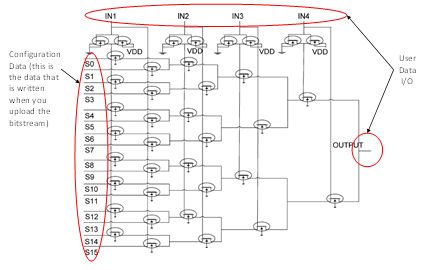
\includegraphics[width=0.8\textwidth]{src/images/6-7.png}
	\caption{4-Input 1-Output Look-Up Table (4-LUT) \cite{Kalenteridis04}}
	\label{fig:fig67}
\end{figure}
\begin{figure}[!htb]
	\centering
	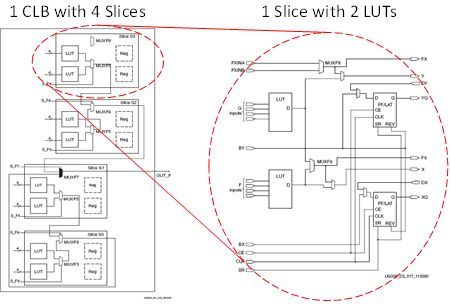
\includegraphics[width=0.8\textwidth]{src/images/6-8.png}
	\caption{CLBs, Slices, and LUTs in a Virtex II FPGA \cite{XUG002}}
	\label{fig:fig68}
\end{figure}
\begin{figure}[!htb]
	\centering
	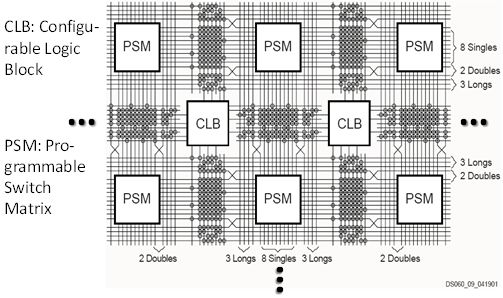
\includegraphics[width=0.8\textwidth]{src/images/6-9.png}
	\caption{ Array of CLBs and PSMs \cite{XDS060}}
	\label{fig:fig69}
\end{figure}
\hypertarget{creating-ise-project-for-getting-accurate-reports}{%
\subsection{Creating ISE Project for Getting Accurate
Reports}\label{creating-ise-project-for-getting-accurate-reports}}

To measure the area and delay of your CPU accurately we designed a new
framework \emph{ISE\_Benchmark}, which consists of four files:
\emph{bram\_dm.ngc}, \emph{brom\_im.ngc}, \emph{dlx\_toplevel.vhd}, and
\emph{dlx\_toplevel.ucf}, which can be found in the directory
``\emph{/home/ces-asip00/­ASIPMeisterProjects/­TEMPLATE\_PROJECT/­ISE\_­Benchmark/}''.
The first two files are BlockRAM netlist files for data and instruction
memories. The VHDL file is the top level for the whole project. The UCF
file is the file, which contains the timing constraints and pins
location for the design (in this step, we specify only the clock and
reset constraints).

Using this framework, all the CPU connections will be mapped to the
FPGA-internal BRAM memory and this will decrease the area needed to
implement the project and will give more accuracy to compute the
processor area and speed. To obtain the area and speed results for your
CPU, your CPU files with this special framework have to be synthesized
and implemented as explained in Chapter~6.1 and Chapter~6.3.

\hypertarget{getting-area-report}{%
\subsection{Getting Area Report}\label{getting-area-report}}

In the Process sub window, expand ``\emph{Place \& Route}'' process.
Double clicking on ``\emph{Place \& Route Report}'' will open new window
containing the results needed. Try to find the number of slices in the
``\emph{Device Utilization Summary}'' as shown in
Figure \ref{fig:fig610}.

\hypertarget{getting-delay-report}{%
\subsection{Getting Delay Report}\label{getting-delay-report}}

In the Process sub window, expand ``\emph{Place \& Route}'' process and
expand ``\emph{Generate Post-Place \& Route Static Timing Report}''.
Double clicking on ``\emph{Text-based Post-Place \& Route Static Timing
Report}'' will open new window containing the results needed. Try to
find minimum Period in the ``\emph{Design Statistics}'' as shown in
Figure \ref{fig:fig611}.
\begin{figure}[!htb]
	\centering
	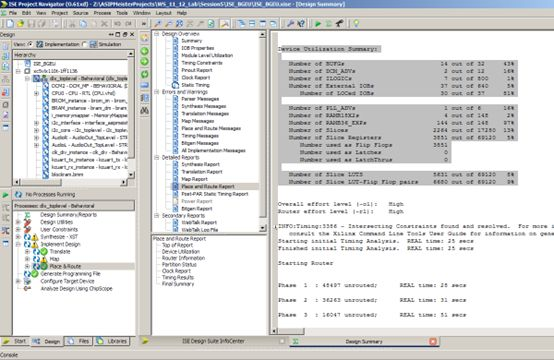
\includegraphics[width=0.9\textwidth]{src/images/6-10.png}
	\caption{Area Report}
	\label{fig:fig610}
\end{figure}
\begin{figure}[!htb]
	\centering
	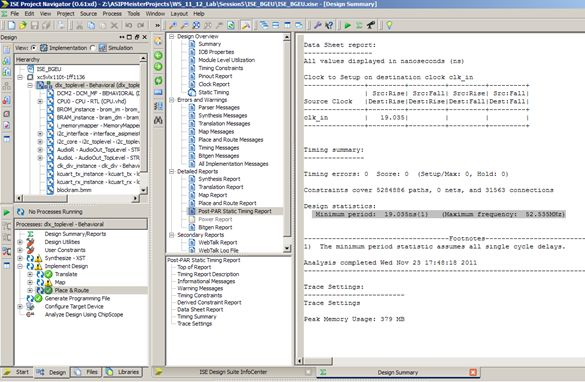
\includegraphics[width=0.9\textwidth]{src/images/6-11.png}
	\caption{Delay Report}
	\label{fig:fig611}
\end{figure}
\hypertarget{getting-critical-path-report}{%
\subsection{Getting Critical Path
Report}\label{getting-critical-path-report}}

To get the critical path, you have to analyze against the timing
constraints. To do that, expand the ``\emph{Place \& Route}'' process in
the sub window \emph{Process}, and then expand ``\emph{Generate
Post-Place \& Route Static Timing Report}''. A double click on
``\emph{Analyze Post-Place\& Route Static Timing (Timing Analyzer)}''
will open a new window for analyzing the timing. In this window, click
on ``\emph{Analyze Analyze against timing constraints}'' as shown in
Figure \ref{fig:fig612}.
\begin{figure}[!htb]
	\centering
	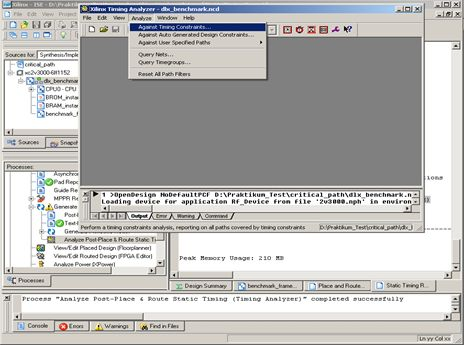
\includegraphics[width=0.9\textwidth]{src/images/6-12.png}
	\caption{Timing Analyzer Window}
	\label{fig:fig612}
\end{figure}
\begin{figure}[!htb]
	\centering
	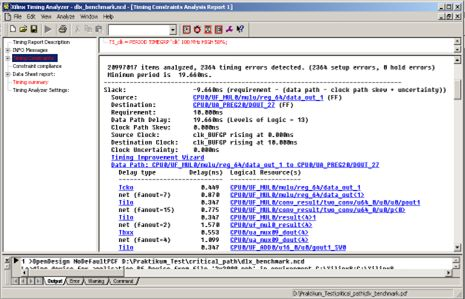
\includegraphics[width=0.9\textwidth]{src/images/6-13.png}
	\caption{Critical Path in the Xilinx Timing Analyzer}
	\label{fig:fig613}
\end{figure}

In the ``\emph{Analyze against timing constraints}'' window, keep
everything as it is and click OK. After a while, the ``\emph{Timing
Analyzer}'' window will be opened. In this window (shown in
Figure \ref{fig:fig613}), click on the ``\emph{Timing
constraint}'' and you will get the critical paths ordered from the
longest to the shorter paths. For each path, you will find the total
delay and the sub-delays for the signals this path consists of.

In the shown example of Figure \ref{fig:fig613}, you can
see, that the path has it's ``\emph{source}'' and ``\emph{destination}''
inside the \emph{CPU0} (i.e. the instantiation of the ASIP Meister CPU,
as it is named in the dlx\_toplevel.vhd). When looking at the detailed
signals this path consists of, you can see, that it starts in the
multiplier of the CPU (MUL0, as it is named in the ``\emph{Resource
Declaration}'' in ASIP Meister), afterwards goes through a multiplexer
(mux09) and then goes to the adder (ADD0, as it is named in the
``\emph{Resource Declaration}'' in ASIP Meister).

When comparing the maximal frequency of two different CPUs you have to
look at the critical paths of both CPUs to understand why maybe the one
CPU is slower than the other or vice versa.
